\chapter{Proposta}
\label{chap:proposta}
%--------------------------------------------------------------------------------
\section{Considerações iniciais}

Neste capítulo está descrita a proposta de pesquisa desse mestrado. Primeiramente, a metodologia para o estudo e implementação da proposta é descrita. A seção de resultados esperados ressalta quais são os resultados que essa pesquisa almeja e, por fim, as atividades que essa dissertação engloba e seu respectivo cronograma são elencados.

%--------------------------------------------------------------------------------
\section{Metodologia}

\begin{description}
 \item[Pesquisa bibliográfica:] \
 
  \begin{enumerate}
\item \underline{Características latentes}: são estudados diversos métodos de pré-processamento de imagens, como filtros de borramento e filtragem, com o objetivo de obter imagens processadas que sejam melhor caracterizadas para a etapa de classificação. O enfoque está em como realçar determinadas características, como, por exemplo, cor e textura, utilizando diversos algoritmos sobre as imagens originais.

\item \underline{Redes neurais}: por representarem o estado da arte da classificação, reconhecimento e localização de objetos, as redes neurais de convolução são estudadas. Pretende-se utilizar a análise dos resultados do seu treinamento para identificar as características relevantes em imagens. Já as máquinas de Boltzmann restritas são redes neurais mais simples, portanto convenientes para a verificação da relevância de uma imagem para o aprendizado.

\item \underline{Desbalanceamento de classes}: esse problema é fundamentado em reconhecimento de padrões, e consiste em lidar com um conjunto de classes que possuem quantidades desiguais de imagens. Deve-se assim pesquisar métodos que visam equilibrar o número de imagens em cada classe.
    
\item \underline{Descritores}: são investigados métodos capazes de descrever as propriedades das imagens, como histograma global de cor (GCH)~\cite{Gonzalez2007}, vetor de coerência de cor (CCV)~\cite{ccv}, classificação de pixels de borda e interior (BIC)~\cite{bic}, auto-correlograma de cor (ACC)~\cite{acc} e descritores de Haralick~\cite{Haralick1973}.

\item \underline{Classificador de padrões}: alguns classificadores fundamentados na literatura para a classificação de imagens são o Naive Bayes, OPF (\textit{Optimum-Path Forest}), KNN (\textit{K-Nearest Neighbor}), SVM (\textit{Support Vector Machines}) e Softmax. A depender da performance do sistema após experimentos um destes será escolhido. É importante destacar que esse não é o foco deste estudo, que tem a maior contribuição na pesquisa do pré-processamento das imagens de forma a obter características relevantes e no rebalanceamento de classes com dados de informação visual.
  \end{enumerate}

 \item[Implementação:] a biblioteca \-OpenCV \cite{Intel2010} será utilizada para as funções gerais de carregar, processar, salvar e classificar imagens. A linguagem de programação para utilizar esta biblioteca e na qual esta pesquisa está sendo implementada é C++. Para a geração de gráficos das medidas estatísticas a linguagem de programação Python é utilizada. O código está disponível em \url{https://bitbucket.org/moacirponti/imagefeatureextraction/overview}. 

 \item[Bases de imagens:] considerando que os objetivos propostos possuem um viés genérico, os experimentos vão ser realizados em diversas coleções de imagens com o objetivo de estabelecer ou refutar as hipóteses levantadas.
 
 Os resultados preliminares foram obtidos utilizando a base de imagens COREL\footnote{Disponível em http://wang.ist.psu.edu/docs/related/}, composta por fotografias que representam as classes: tribos africanas, praia, construções, ônibus, dinossauros, elefantes, flores, cavalos, montanhas e tipos de comidas. São 10 classes balanceadas com 100 imagens cada. Para fins de exemplificação, foram selecionadas imagens que representam essas classes na Figura \ref{fig:corel}. 
 
 \begin{figure}[hbpt]
 \begin{center}
   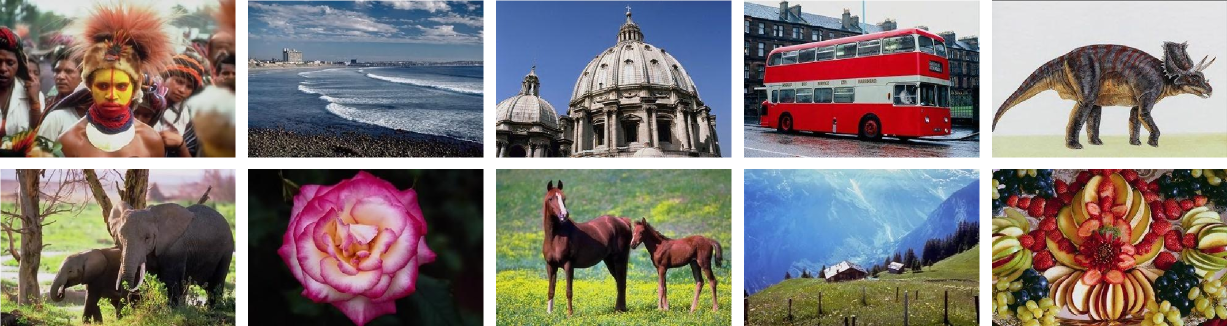
\includegraphics[width=1\linewidth]{\detokenize {figuras/exemplos_corel.png}}
 \end{center}
  \caption[Base de imagens COREL-1000.]{Base de imagens COREL-1000 utilizada. Estão representadas as 10 classes da base. \textit{Fonte: Elaborado pelo autor.}}
 \label{fig:corel}
\end{figure}

 
 \item[Experimentos:] serão realizados diversos experimentos direcionados a explorar as etapas de pré-processamento, para melhorar a acurácia da classificação de bases de imagens. Como entrada são utilizadas imagens originais provenientes de diversas coleções disponíveis na literatura. Como resultado, serão calculadas medidas estatísticas da classificação dessas coleções após a alteração dessas imagens com os métodos de realce de características relevantes.
 
 \item[Análise dos dados:] os experimentos realizados irão resultar em medidas estatísticas da classificação. A análise irá comparar a classificação das imagens originais com aquelas tratadas pelo método proposto. Ainda, o método de rebalanceamento de classes será comparado com técnicas disponíveis na literatura, como o SMOTE.

\item[Forma de avaliação:] a medida estatística mais comum para avaliação é a razão do número de acertos pela quantidade de imagens testadas. Essa medida, conhecida por \underline{acurácia}, pode não refletir propriamente os resultados, em um cenário de bases desbalanceadas. Isso se deve ao fato de que se a classe minoritária não obtiver nenhum resultado correto e a classe majoritária tiver 100\% de acertos, a acurária normal poderá ser muito alta, mesmo considerando que nenhuma imagem da classe minoritária foi corretamente classificada. Dessa forma, considera que os erros são igualmente importantes. Mas em se tratando de bases desbalanceadas, deve-se diferenciar o erro em, por exemplo, diagnosticar um paciente doente -- classe minoritária -- como sendo saudável e um paciente saudável -- classe majoritária -- como estando doente \cite{Batista2004}. No primeiro caso, o paciente corre risco de diagnóstico tardil, enquanto o paciente saudável realiza outros testes para refutação.

Pode-se estender essa medida obtendo-se a \underline{acurácia $k$-fold}: medida de acerto baseada na divisão do conjunto de objetos em teste e treinamento, realizando a repetição dos experimentos $n$ vezes e obtendo a média e o desvio padrão. A acurácia de cada experimento é obtida pela Equação~\ref{eq:Accuracy}, que considera problemas de desbalanceamento de classes.

    \begin{equation}
      Acc = 1 - \frac{\sum_{i=1}^{c} E(i)}{2c},
    \label{eq:Accuracy}
    \end{equation}

    \noindent onde $c$ é o número de classes e $E(i) = e_{i,1} + e_{i,2}$ é o erro relativo a $c$, calculado por:

    \begin{equation*}
      e_{i,1} = \frac{FP(i)}{N-N(i)} \,\,\,\,\, \text{ e } \,\,\,\,\, e_{i,2} = \frac{FN(i)}{N(i)}, i=1,...,c,
    \label{eq:Errors}
    \end{equation*}
   \noindent onde $FN(i)$ (falsos negativos) são os exemplos pertencentes a $i$ e incorretamente classificados, e $FP(i)$ (falsos positivos) são os exemplos erroneamente rotulados como~$i$.

% consideramos positivos a minoritaria

Uma outra medida para bases desbalanceadas é a \underline{medida-F1} (conhecida como \textit{F1-Measure} ou \textit{F1-Score} e apresentada na Equação~\eqref{medidaf}), que combina precisão e revocação como medida de efetividade da classificação \cite{Garcia2009}. 
% Pode efetivamente avaliar a performance de classificação em cenários desbalanceados. 
A precisão (Equação~\ref{precisao}) é a medida da exatidão: dos exemplos classificados como positivos, quantos realmente são. E a revocação (Equação~\ref{revocacao}) é a medida de completude: quantos exemplos positivos foram corretamente classificados como tal. 

\begin{equation}
  P = \frac{VP}{VP + FP},
  \label{precisao}
\end{equation}

\noindent onde $VP$ são os exemplos positivos corretamente classificados.

\begin{equation}
  R = \frac{VP}{VP + FN}
  \label{revocacao}
\end{equation}

\begin{equation}
  F1 = 2 \frac{PR}{P+R}
  \label{medidaf}
\end{equation}

A partir dessas medidas, o \underline{teste estatístico de Friedman} pode ser usado para determinar se há diferença significante em uma amostra de resultados gerados \cite{friedman2010}. As performances dos algoritmos são analisados e um \textit{rank} é atribuído para cada conjunto de dados. Ele considera que a hipótese nula a ser testada é que não há diferença estatística relevante entre as observações. Para analisar se o teste da hipótese é significativo, pode ser utilizado o \underline{p-valor}, que indica o quão estatisticamente significante o resultado é: quanto menor o seu valor, maior a evidência contra a hipótese nula (geralmente o limiar utilizado é de 0,05).

Por fim, a \underline{distância de Mahalanobis} também pode ser utilizada: antes e depois da geração artificial de imagens, calcular a distância entre a média das classes e a variância dentro das classes \cite{mahalanobis2000}. Ela se baseia na correlação entre as variáveis e pode ser definida por
\begin{equation*}
  D_m(x_i) = \sqrt{(x_i - \mu)C^{-1}(x_i-\mu)^T},
\end{equation*}
\noindent onde $x_i$ é um vetor de valores, $\mu$ a média e C a matriz de covariância.

\end{description}

%--------------------------------------------------------------------------------
\section{Resultados esperados}
\label{sec:resultados}

Os resultados esperados são relacionados às áreas de \textbf{processamento de imagens e reconhecimento de padrões}. Espera-se obter uma comprovação das hipóteses levantadas por essa pesquisa. Os resultados são esperados em duas vertentes:

\begin{enumerate}
 \item \textit{Pré-processamento} de imagens que caracterizem melhor aspectos de suas classes, aumentando a variância entre as classes quando comparado com as imagens originais.
 \item \textit{Geração artificial de imagens} de classes minoritárias de forma a compensar o desbalanceamento natural das bases de dados.
\end{enumerate}

Em ambos os casos pretende-se melhorar a classificação, validando-a através do cálculo da medida-F1. A análise das características aprendidas por uma rede neural de convolução será realizada ao executar o treinamento com bases específicas que destaquem propriedades como cor, textura e forma. Além disso, os resultados serão obtidos a partir da escolha de quais imagens adicionam informação ao conjunto de treino. As redes RBM serão utilizadas para este fim. Bases naturalmente não balanceadas serão testadas e seus resultados avaliados.

%--------------------------------------------------------------------------------
\section{Atividades e cronograma previsto}

As principais atividades contempladas no desenvolvimento dessa pesquisa de mestrado são as seguintes:

\begin{enumerate}
 \item Integralização dos créditos das disciplinas do Programa de Mestrado do ICMC/USP;
 \item Revisão bibliográfica;
 \item Estudo e implementação da geração de imagens artificiais para corrigir o desbalanceamento de classes;
 \item Estudo e implementação de métodos para obtenção de características latentes;
 \item Projetar e realizar experimentos com diversas bases de dados utilizando os métodos propostos e posterior validação;
 \item Escrita científica para a produção do exame de qualificação, dissertação de mestrado e artigos científicos.
\end{enumerate}

% \setlength{\tabcolsep}{0pt}
\begin{table} \label{t:atividades}
\caption{Duração de cada atividade a partir de 24/02/2014.}
\begin{center}
\begin{tabular}{|c|c|c|c|c|c|}
 \cline{2-6}
\multicolumn{1}{l|}{} & \multicolumn{2}{c|}{2014} & \multicolumn{2}{c|}{2015} & 2016 \\
\hline \ Atividade\ \ & 1\textordmasculine\ Sem. & 2\textordmasculine\
Sem. & 1\textordmasculine\ Sem. & 2\textordmasculine\ Sem. & 1\textordmasculine\ Sem. \\
\hline \hline
%                           &       2014        &       2015         \\
1   &\y\y    &\y\y      &\x\x     &\x\x    &\x    \\
\hline
2   &\x\x    &\y\y      &\r\r     &\r\r    &\x    \\
\hline
3   &\x\x    &\y\y      &\r\r     &\r\x    &\x    \\
\hline
4   &\x\x    &\x\x      &\x\r     &\r\r    &\x    \\
\hline
5   &\x\x    &\x\y      &\r\r     &\r\r    &\x    \\
\hline
6   &\x\x    &\x\y      &\r\x     &\x\r    &\r\x  \\
\hline
\end{tabular}
\end{center}
\end{table}

%--------------------------------------------------------------------------------
\section{Considerações finais}

A proposta desta pesquisa foi apresentada, descrevendo a sua metodologia. Foi dado destaque aos resultados esperados e à forma de avaliação, descrevendo as medidas estatísticas a serem utilizadas. O cronograma previsto para a realização deste mestrado foi destacado, elencando as atividades e suas respetivas durações. O próximo capítulo apresentará os resultados preliminares.